% ============================================================
% Defesa de TCC — Previsão de Rebaixamento no Brasileirão Série A
% Leonardo Feitosa Barroso $\cdot$ UFPB/CCSA $\cdot$ Ciência de Dados para Negócios
%
% Compilar: tectonic apresentacao.tex     (ou xelatex/pdflatex 2x)
% Alvo: ~13-14 min de fala + ~5 min de demonstração do app.
%
% Notas de manutenção:
%  $\cdot$ "\\" dentro de nó TikZ com align=center quebra nesta versão do TikZ;
%    por isso os nós usam \parbox + \par (ver \tile, \faixa, \pcx).
%  $\cdot$ \newcommand com parâmetro precisa ficar no preâmbulo: em corpo de
%    frame Beamer exigiria "##1" e quebra o \foreach do TikZ.
% ============================================================
% 11pt: o frametitle customizado (com subtítulo + fio) consome altura que o
% Beamer não contabiliza em \textheight; 11pt devolve a folga necessária.
\documentclass[aspectratio=169,11pt,t]{beamer}

\usepackage[utf8]{inputenc}
\usepackage[T1]{fontenc}
\usepackage{lmodern}
\usepackage{textcomp}
\providecommand{\euro}{\texteuro}
\usepackage[brazil]{babel}
\usepackage{graphicx}
\usepackage{tikz}
\usepackage{amsmath}
\usetikzlibrary{positioning, arrows.meta}

\graphicspath{{figuras/}}

% ── Paleta (validada para daltonismo: Okabe-Ito) ────────────────────────────
\definecolor{azul}{HTML}{0072B2}      % Reg. Logística / protege
\definecolor{verm}{HTML}{D55E00}      % LightGBM / risco
\definecolor{verde}{HTML}{009E73}     % Random Forest
\definecolor{roxo}{HTML}{CC79A7}      % XGBoost
\definecolor{tinta}{HTML}{262B30}
\definecolor{tinta2}{HTML}{5A646E}
\definecolor{fundoc}{HTML}{EDF1F4}

% ── Tema minimalista próprio ────────────────────────────────────────────────
\usetheme{default}
\usecolortheme{default}
\setbeamertemplate{navigation symbols}{}
\setbeamercolor{normal text}{fg=tinta}
\setbeamercolor{frametitle}{fg=azul}
\setbeamercolor{structure}{fg=azul}
\setbeamerfont{frametitle}{size=\large, series=\bfseries}
\setbeamerfont{framesubtitle}{size=\footnotesize}
\setbeamercolor{framesubtitle}{fg=tinta2}
\setbeamertemplate{itemize item}{\color{azul}\rule[0.25ex]{0.45ex}{0.45ex}}
\setbeamerfont{itemize/enumerate body}{size=\normalsize}
\setbeamerfont{itemize/enumerate subbody}{size=\small}

\makeatletter
\setbeamertemplate{frametitle}{%
    \vspace{0.35em}%
    \begin{beamercolorbox}[wd=\paperwidth,leftskip=0.9cm,rightskip=0.9cm]{frametitle}%
        \insertframetitle%
        \ifx\insertframesubtitle\@empty\else
            \\[0.1em]{\usebeamerfont{framesubtitle}\usebeamercolor[fg]{framesubtitle}\insertframesubtitle}%
        \fi
    \end{beamercolorbox}%
    \vspace{-0.25em}%
    \hspace{0.9cm}\textcolor{azul!30}{\rule{\dimexpr\paperwidth-1.8cm\relax}{0.8pt}}%
}
\makeatother

\setbeamertemplate{footline}{%
    \hspace{0.9cm}\textcolor{tinta2}{\scriptsize Previsão de rebaixamento --- Brasileirão Série A}%
    \hfill%
    \textcolor{tinta2}{\scriptsize\insertframenumber/\inserttotalframenumber}%
    \hspace{0.9cm}\vspace{0.25cm}%
}
\setbeamersize{text margin left=0.9cm, text margin right=0.9cm}

% ── Atalhos ─────────────────────────────────────────────────────────────────
\newcommand{\chave}[1]{%
    \begin{center}
        \begin{minipage}{0.88\textwidth}
            \centering\Large\bfseries\color{azul} #1
        \end{minipage}
    \end{center}
}

% Cartão de número
\newcommand{\tile}[3]{%
    \begin{tikzpicture}[baseline]
        \node[rounded corners=4pt, fill=fundoc, inner sep=6pt,
              minimum width=2.75cm] {%
            \parbox{2.55cm}{\centering
                {\fontsize{20}{22}\selectfont\bfseries\color{#1} #2}\par
                \vspace{0.2em}
                {\scriptsize\color{tinta2} #3}}%
        };
    \end{tikzpicture}%
}

% Faixa de destaque
\newcommand{\faixa}[2]{%
    \begin{tikzpicture}
        \node[rounded corners=4pt, fill=#1!12, inner sep=7pt] {%
            \parbox{\dimexpr\textwidth-26pt\relax}{\centering
                \normalsize\bfseries\color{#1} #2}%
        };
    \end{tikzpicture}%
}

\newcommand{\fonte}[1]{{\scriptsize\color{tinta2} #1}}
\newcommand{\pcx}[1]{\parbox{1.55cm}{\centering\tiny #1}}
\newcommand{\marca}[1]{\textcolor{#1}{\rule[0.25ex]{1ex}{1ex}}}

% ============================================================
\begin{document}

% ── 1. Capa ────────────────────────────────────────────────────────────────
{
\setbeamertemplate{footline}{}
\begin{frame}[plain]
    \vspace{0.5cm}
    \begin{center}
        
\includegraphics[height=1.25cm]{../../tcc_artigo/figuras/brasao_ufpb.png}

        \vspace{0.25cm}
        {\scriptsize\color{tinta2} UNIVERSIDADE FEDERAL DA PARAÍBA --- CCSA\\
        Bacharelado em Ciência de Dados para Negócios}

        \vspace{0.7cm}
        {\Large\bfseries\color{azul} Previsão de Rebaixamento no\\ Campeonato Brasileiro Série A}

        \vspace{0.25em}
        {\small\color{tinta2} Uma comparação de modelos de \emph{Machine Learning}\\ com validação \emph{walk-forward}}

        \vspace{0.65cm}
        {\normalsize\bfseries Leonardo Feitosa Barroso}\\[0.15em]
        {\scriptsize\color{tinta2} Orientador: Prof. Dr. Hilton Martins de Brito Ramalho}

        \vspace{0.45cm}
        {\scriptsize\color{tinta2} João Pessoa $\cdot$ \the\year}
    \end{center}
\end{frame}
}

% ── 2. Roteiro ─────────────────────────────────────────────────────────────
\begin{frame}{Roteiro}
    \vspace{0.5cm}
    \begin{columns}[t]
        \begin{column}{0.5\textwidth}
            \begin{enumerate}
                \item[\textcolor{azul}{\textbf{1}}] O problema e a pergunta
                \item[\textcolor{azul}{\textbf{2}}] Dados e método
                \item[\textcolor{azul}{\textbf{3}}] Resultados
            \end{enumerate}
        \end{column}
        \begin{column}{0.5\textwidth}
            \begin{enumerate}
                \item[\textcolor{azul}{\textbf{4}}] A prova real: 2025
                \item[\textcolor{azul}{\textbf{5}}] Contribuições e limites
                \item[\textcolor{verm}{\textbf{6}}] \textbf{Demonstração do app}
            \end{enumerate}
        \end{column}
    \end{columns}
\end{frame}

% ── 3. O problema ──────────────────────────────────────────────────────────
\begin{frame}{O problema}
    \framesubtitle{Cair para a Série B é o pior resultado financeiro possível para um clube}
    \vspace{0.35cm}
    \begin{center}
        \tile{verm}{4}{clubes rebaixados\par por temporada}\hfill
        \tile{verm}{20\%}{das observações\par --- classe minoritária}\hfill
        \tile{azul}{$-$}{receita de TV,\par patrocínio e elenco}
    \end{center}

    \vspace{0.45cm}
    \begin{itemize}\itemsep0.25em
        \item A queda derruba receitas de transmissão, patrocínios e o valor do elenco.
        \item Os efeitos se arrastam por \textbf{várias temporadas}.
        \item Antecipar o risco permite agir: reforços, renegociação, orçamento.
    \end{itemize}
\end{frame}

% ── 4. A pergunta ──────────────────────────────────────────────────────────
\begin{frame}{A pergunta}
    \vspace{0.5cm}
    \chave{Dá para estimar quem cai\\ \emph{antes de a bola rolar}?}

    \vspace{0.55cm}
    \begin{itemize}\itemsep0.25em
        \item A literatura foca em \textbf{resultado de partidas} e em \textbf{ligas europeias}.
        \item Não localizei trabalho sobre rebaixamento no Brasileirão usando
              \textbf{apenas informação pré-temporada}.
        \item É justamente o cenário em que a previsão \textbf{serve para decidir algo}.
    \end{itemize}

    \vspace{0.3cm}
    \fonte{Busca no Google Scholar e Scopus: (\emph{relegation} OR rebaixamento) AND (\emph{machine learning} OR \emph{prediction}).}
\end{frame}

% ── 5. Dados ───────────────────────────────────────────────────────────────
\begin{frame}{Os dados}
    \framesubtitle{Transfermarkt, raspagem automatizada $\cdot$ dados públicos, uso acadêmico}
    \vspace{0.3cm}
    \begin{center}
        \tile{azul}{220}{observações rotuladas\par (2014--2024)}\hfill
        \tile{azul}{15}{variáveis preditoras\par (\emph{features})}\hfill
        \tile{verm}{2025}{temporada reservada\par para prever}
    \end{center}

    \vspace{0.4cm}
    \begin{columns}[t]
        \begin{column}{0.47\textwidth}
            \small\textbf{\color{azul}3 de elenco} \emph{(o que o clube tem)}
            \begin{itemize}\small\itemsep0.1em
                \item valor de mercado
                \item tamanho do plantel
                \item n.\textordmasculine{} de estrangeiros
            \end{itemize}
        \end{column}
        \begin{column}{0.47\textwidth}
            \small\textbf{\color{azul}12 de janela deslizante} \emph{(o que ele fez)}
            \begin{itemize}\small\itemsep0.1em
                \item médias de 3 e 5 temporadas
                \item pontos, saldo, gols, vitórias, aproveitamento
            \end{itemize}
        \end{column}
    \end{columns}
\end{frame}

% ── 6. O método ────────────────────────────────────────────────────────────
\begin{frame}{O método}
    \framesubtitle{Um fio condutor: nenhuma informação do futuro entra no modelo}
    \vspace{0.7cm}
    \begin{center}
    \begin{tikzpicture}[
        node distance=0.28cm,
        cx/.style={rounded corners=3pt, draw=azul!45, fill=azul!8, inner sep=5pt},
        fl/.style={-{Stealth[length=3.5pt]}, azul!60, thick}]
        \node[cx] (a) {\pcx{Coleta\par Transfermarkt}};
        \node[cx, right=of a] (b) {\pcx{Janelas\par \texttt{shift(1)}\par \texttt{.rolling()}}};
        \node[cx, right=of b] (c) {\pcx{Imputação e\par padronização\par \textbf{só no treino}}};
        \node[cx, right=of c] (d) {\pcx{Validação\par \emph{walk-}\par \emph{forward}}};
        \node[cx, right=of d] (e) {\pcx{Ajuste de\par hiperpar.}};
        \node[cx, right=of e] (f) {\pcx{Teste\par 2023--24}};
        \foreach \x/\y in {a/b, b/c, c/d, d/e, e/f} \draw[fl] (\x) -- (\y);
    \end{tikzpicture}
    \end{center}

    \vspace{0.7cm}
    \begin{center}
        \faixa{verm}{As médias da temporada $T$ usam só $T-1$ a $T-w$. Nunca a própria temporada prevista.}
    \end{center}
\end{frame}

% ── 7. Por que walk-forward ────────────────────────────────────────────────
\begin{frame}{Por que não a validação cruzada tradicional?}
    \vspace{0.45cm}
    \begin{columns}[t]
        \begin{column}{0.47\textwidth}
            \small\textbf{\color{roxo}$k$-fold embaralhado}

            \vspace{0.3cm}
            \begin{tikzpicture}[y=0.45cm, x=0.28cm]
                \foreach \i/\c in {0/roxo,1/gray,2/roxo,3/gray,4/roxo,5/gray,6/roxo,7/gray,8/roxo,9/gray,10/roxo}
                    \fill[\c!55, rounded corners=1pt] (\i,0) rectangle (\i+0.78,0.7);
            \end{tikzpicture}

            \vspace{0.1cm}
            \fonte{2014 $\rightarrow$ 2024, ordem embaralhada}

            \vspace{0.35cm}
            {\small Treina com temporadas \textbf{futuras} para prever o passado.}

            \vspace{0.2cm}
            {\small\color{roxo}\textbf{Otimista e irreal.}}
        \end{column}
        \begin{column}{0.47\textwidth}
            \small\textbf{\color{azul}\emph{Walk-forward} (janela expansiva)}

            \vspace{0.3cm}
            \begin{tikzpicture}[y=0.28cm, x=0.28cm]
                \foreach \r/\n in {0/5, 1/6, 2/7, 3/8, 4/9} {
                    \foreach \i in {0,...,\n}
                        \fill[azul!55, rounded corners=1pt] (\i,-\r*1.3) rectangle (\i+0.78,-\r*1.3+0.85);
                    \pgfmathtruncatemacro{\v}{\n+1}
                    \fill[verm!75, rounded corners=1pt] (\v,-\r*1.3) rectangle (\v+0.78,-\r*1.3+0.85);
                }
            \end{tikzpicture}

            \vspace{0.15cm}
            \fonte{treino \marca{azul!55} \quad validação \marca{verm!75}}

            \vspace{0.25cm}
            {\small Sempre treina no passado e valida no ano seguinte.}
        \end{column}
    \end{columns}
\end{frame}

% ── 8. Walk-forward: resultado ─────────────────────────────────────────────
\begin{frame}{Estabilidade ao longo das temporadas}
    \framesubtitle{AUC-ROC em cada temporada de validação --- 5 partições}
    \vspace{0.1cm}
    \begin{center}
        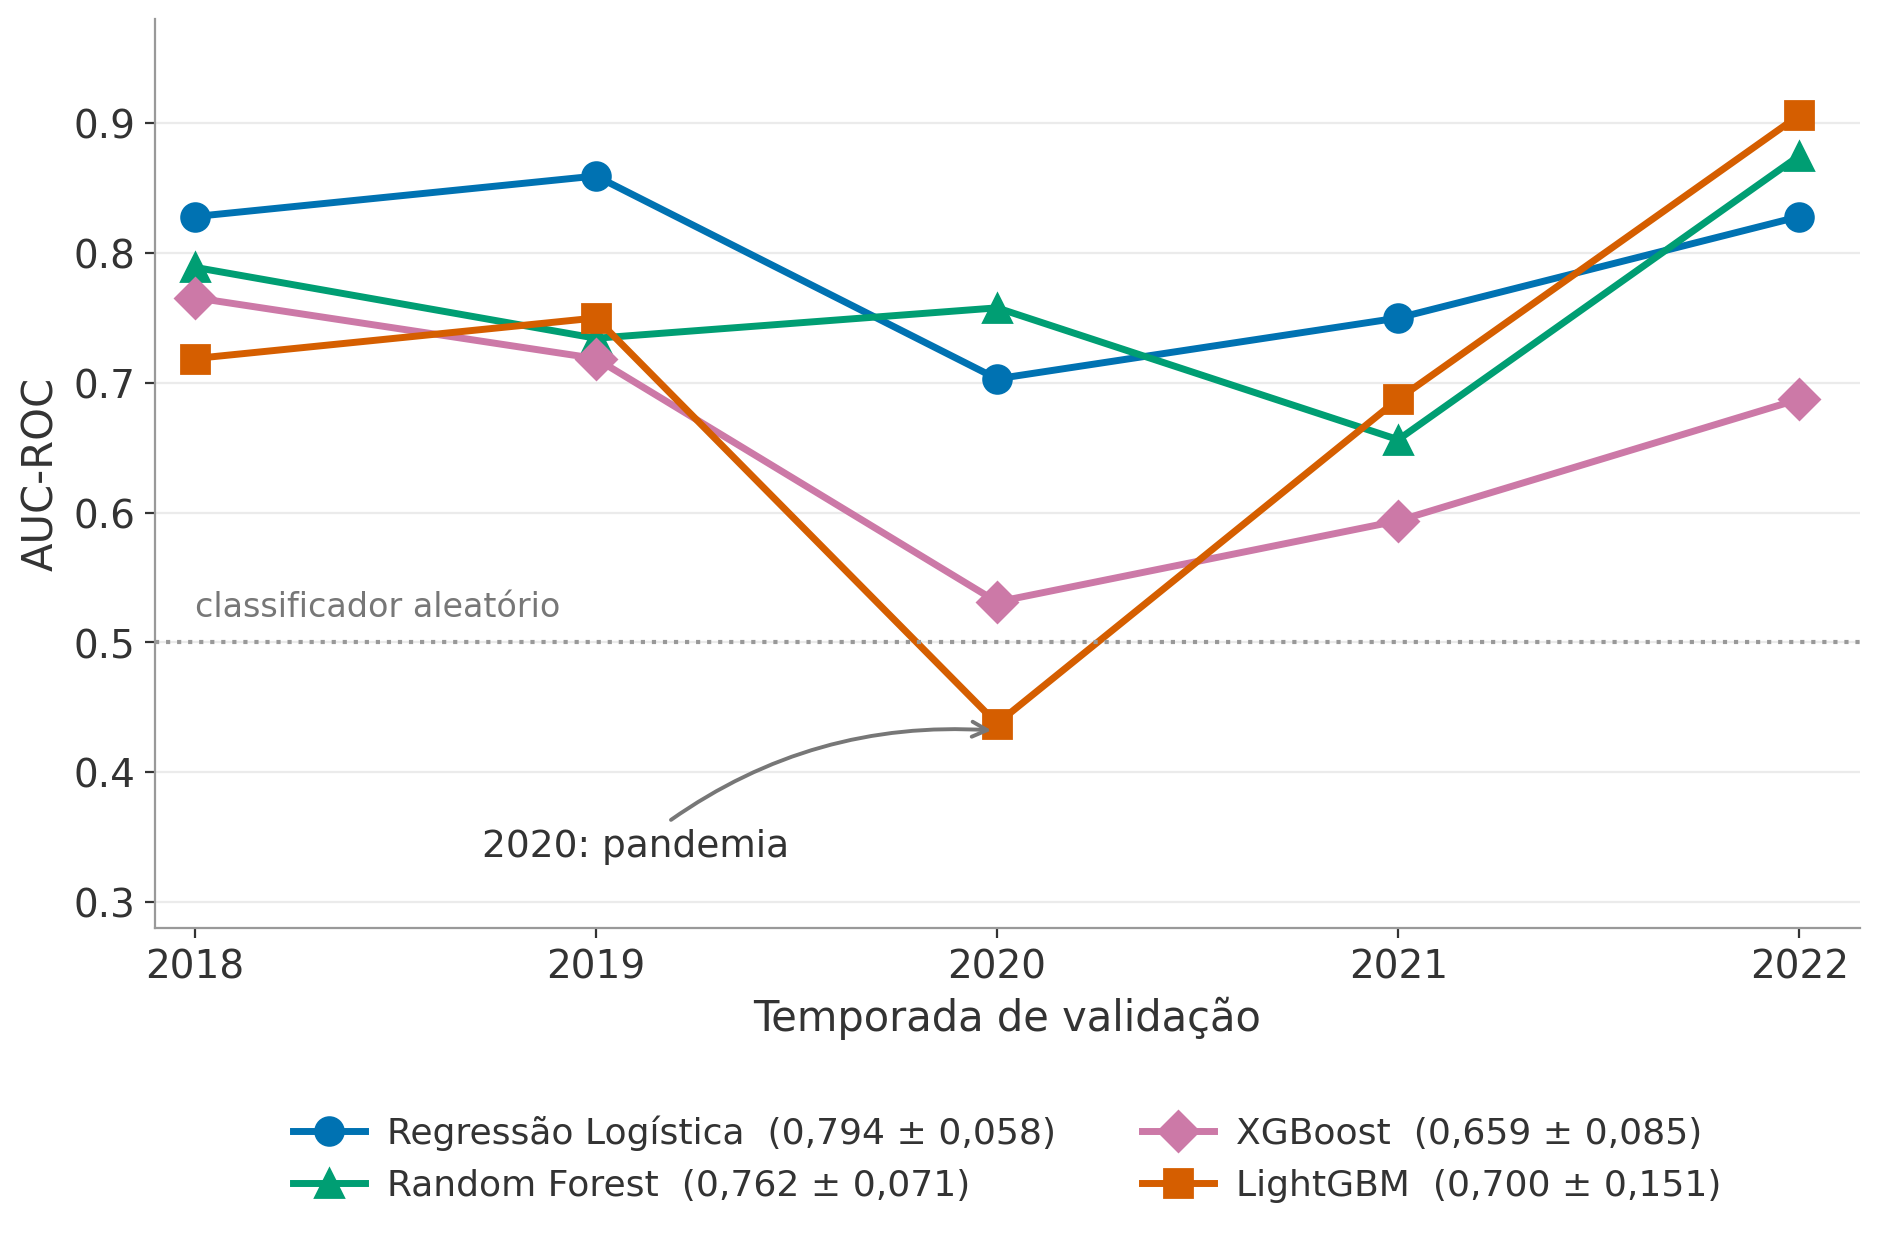
\includegraphics[height=0.60\textheight]{slide_walkforward.png}
    \end{center}
    \begin{center}
        \small A Regressão Logística é a \textbf{mais estável} ($\pm$0,058);
        o LightGBM, o \textbf{mais volátil} ($\pm$0,151).
    \end{center}
\end{frame}

% ── 9. Teste independente ──────────────────────────────────────────────────
\begin{frame}{Teste independente: 2023--2024}
    \framesubtitle{40 observações nunca vistas em nenhuma etapa anterior}
    \vspace{0.15cm}
    \begin{columns}[c]
        \begin{column}{0.54\textwidth}
            \begin{center}
                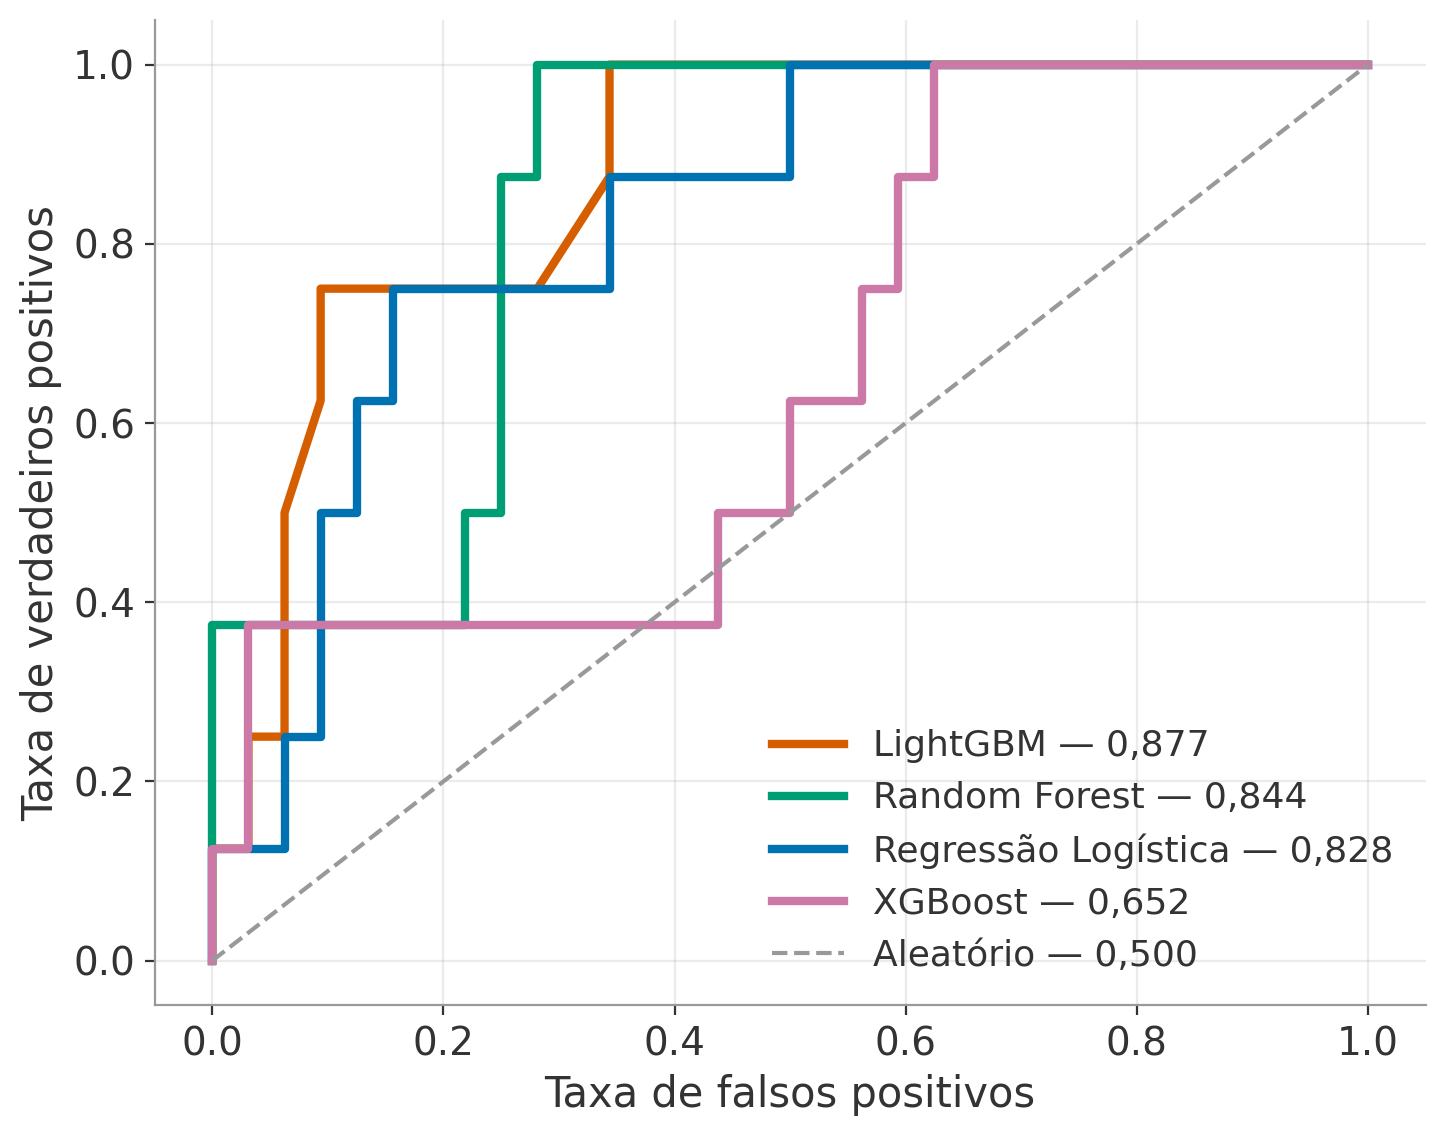
\includegraphics[height=0.60\textheight]{slide_roc.png}
            \end{center}
        \end{column}
        \begin{column}{0.43\textwidth}
            \small
            \marca{verm}~ \textbf{LightGBM 0,877}\\[0.35em]
            \marca{verde}~ Random Forest 0,844\\[0.35em]
            \marca{azul}~ Reg. Logística 0,828\\[0.35em]
            \marca{roxo}~ XGBoost \textbf{0,652}

            \vspace{0.7cm}
            {\normalsize\color{verm}\textbf{Mas o XGBoost tem a mesma acurácia que o LightGBM: 82,5\%.}}
        \end{column}
    \end{columns}
\end{frame}

% ── 10. A armadilha da acurácia ────────────────────────────────────────────
\begin{frame}{A armadilha da acurácia}
    \framesubtitle{Mesma acurácia, mesma matriz de confusão --- AUC muito diferente}
    \vspace{0.15cm}
    \begin{center}
        \small
        \marca{roxo}~XGBoost \textbf{82,5\%} $\to$ AUC \textbf{0,652}
        \hspace{1.1cm}
        \marca{verm}~LightGBM \textbf{82,5\%} $\to$ AUC \textbf{0,877}
    \end{center}

    \vspace{0.1cm}
    \begin{center}
        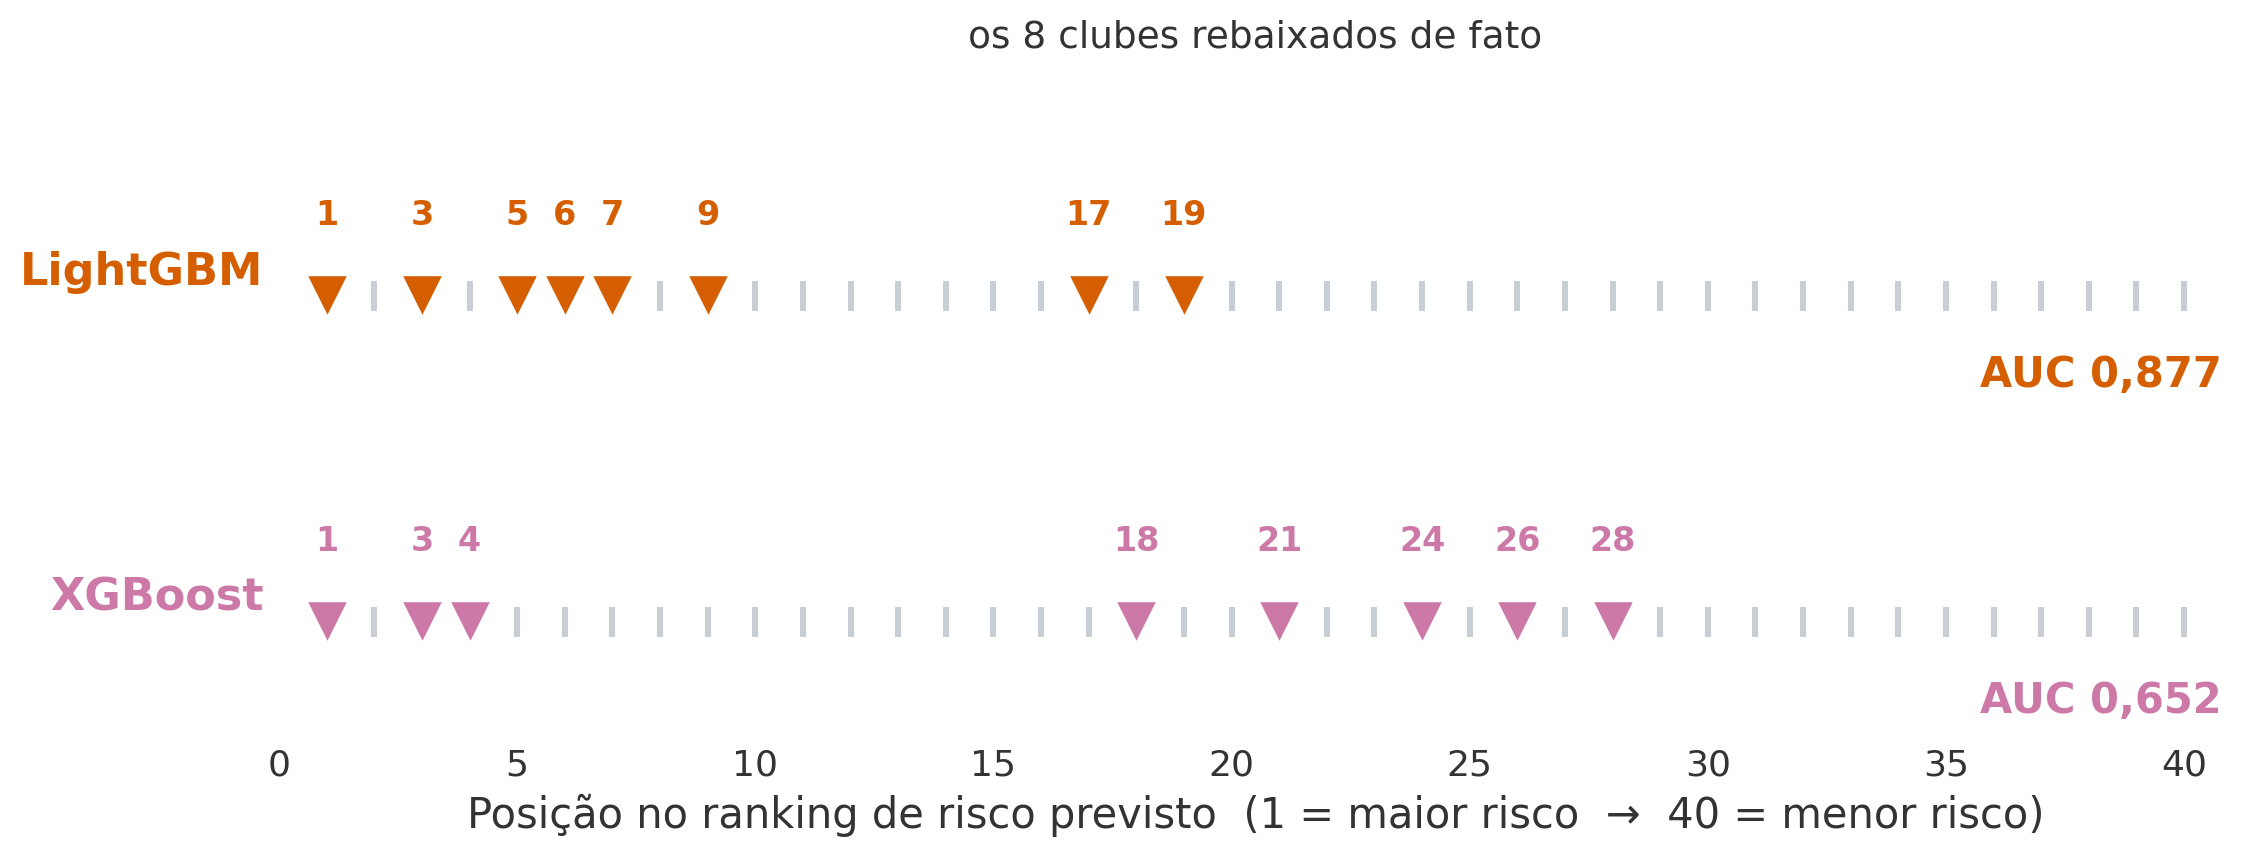
\includegraphics[height=0.45\textheight]{slide_armadilha.png}
    \end{center}

    \vspace{0.1cm}
    \begin{center}
        \small A acurácia só olha a decisão no limiar. O AUC olha a
        \textbf{ordenação inteira} --- e é ela que serve à gestão.
    \end{center}
\end{frame}

% ── 11. O que pesa ─────────────────────────────────────────────────────────
\begin{frame}{O que pesa no risco}
    \framesubtitle{Coeficientes padronizados da Regressão Logística --- 8 maiores em módulo}
    \vspace{0.1cm}
    \begin{center}
        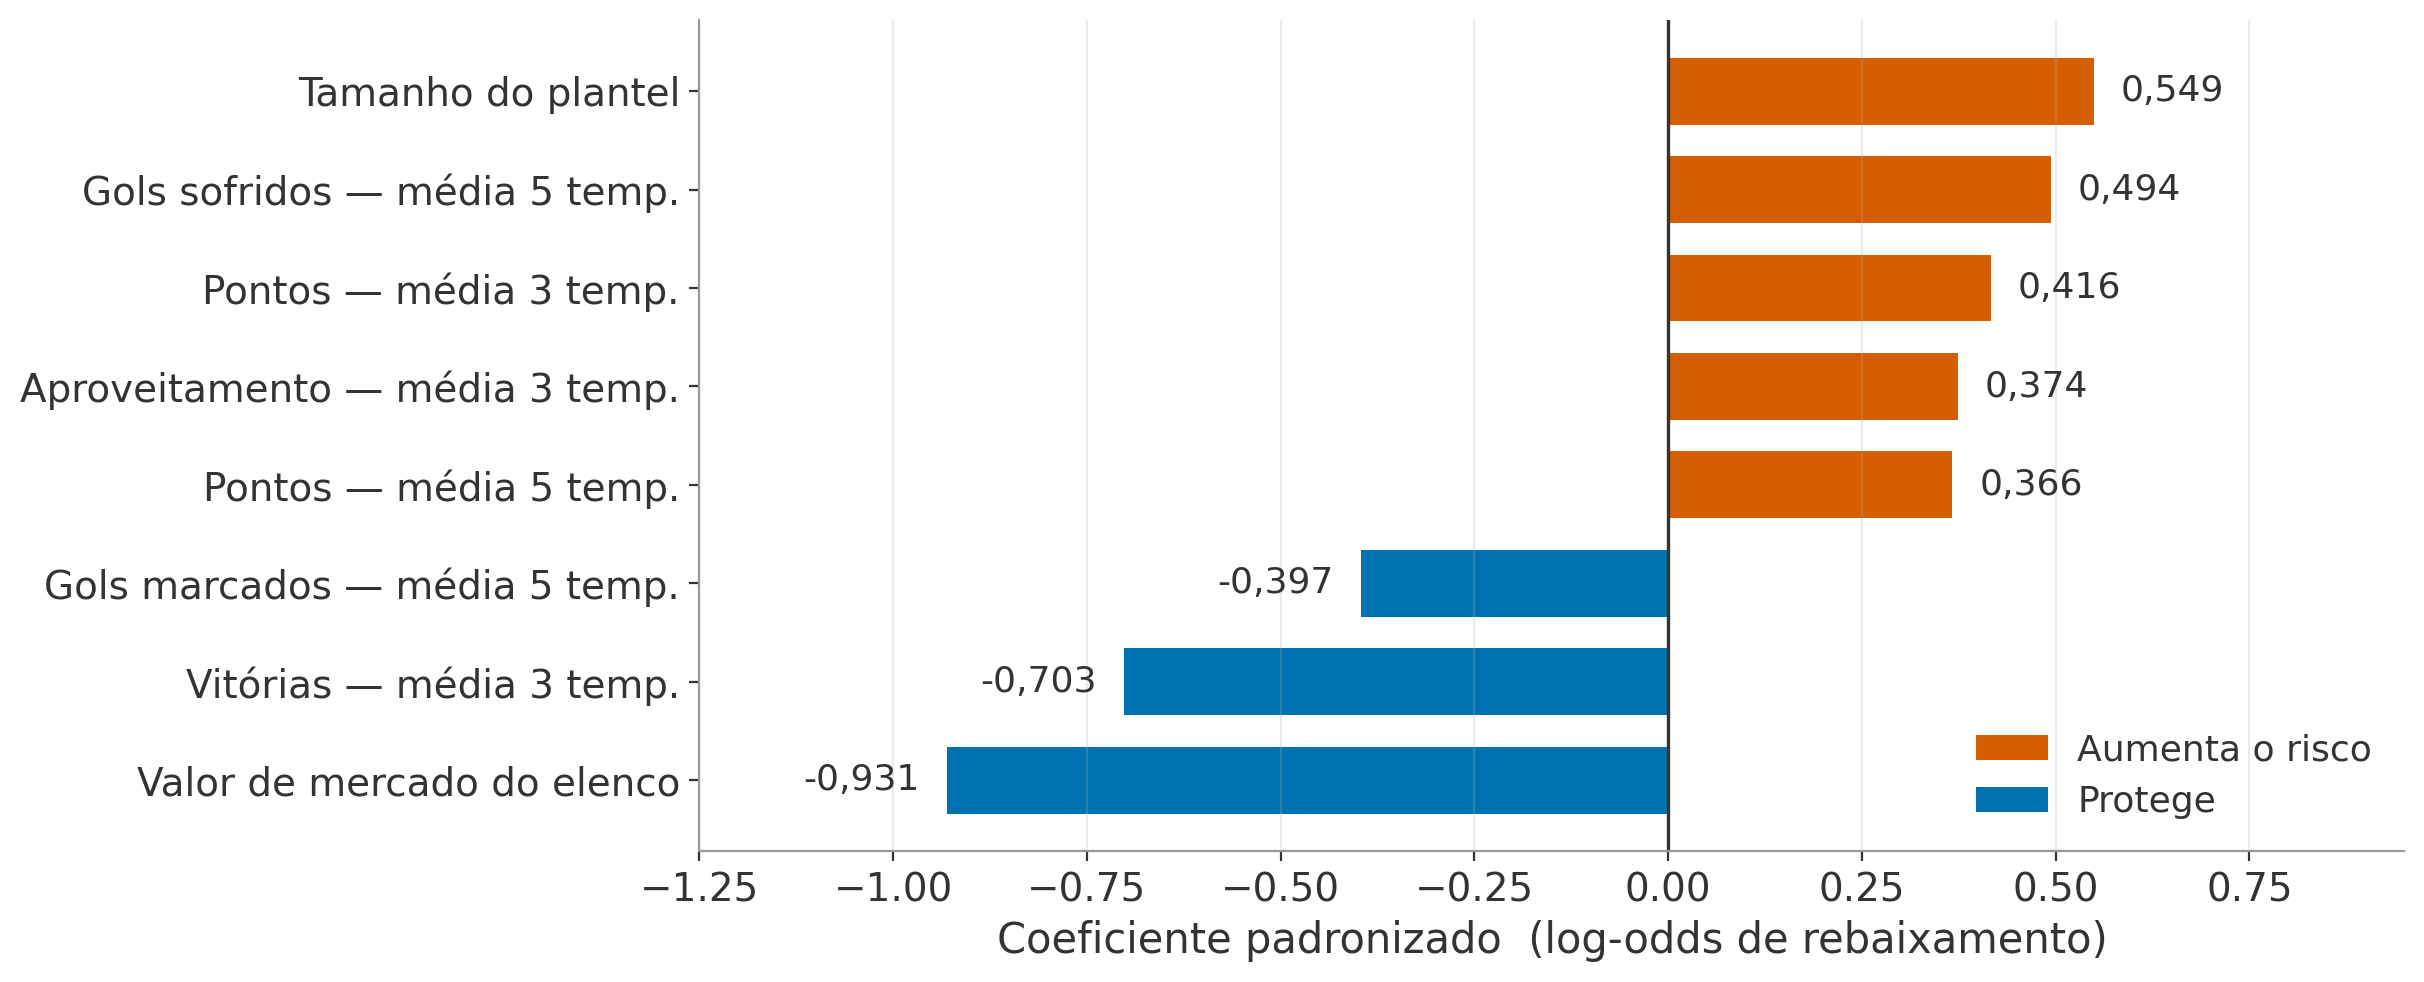
\includegraphics[height=0.57\textheight]{slide_importancia.png}
    \end{center}
    \begin{center}
        \small \textbf{Valor de elenco é a variável dominante}; vitórias recentes protegem.
    \end{center}
\end{frame}

% ── 12. Modelo final ───────────────────────────────────────────────────────
\begin{frame}{Qual modelo levar para a prática?}
    \vspace{0.5cm}
    \begin{columns}[t]
        \begin{column}{0.47\textwidth}
            \textbf{\color{verm}LightGBM}
            \begin{itemize}\itemsep0.2em
                \item melhor AUC no teste: \textbf{0,877}
                \item mas oscila entre temporadas: $\pm$0,151
                \item caixa-preta
            \end{itemize}
        \end{column}
        \begin{column}{0.47\textwidth}
            \textbf{\color{azul}Regressão Logística}
            \begin{itemize}\itemsep0.2em
                \item AUC 0,828 --- terceira
                \item \textbf{mais estável}: $\pm$0,058
                \item coeficientes interpretáveis
                \item probabilidades calibradas
            \end{itemize}
        \end{column}
    \end{columns}

    \vspace{0.7cm}
    \begin{center}
        \faixa{azul}{Escolhi a Regressão Logística: estabilidade e interpretabilidade acima do pico de desempenho.}
    \end{center}
\end{frame}

% ── 13. Previsão 2025 ──────────────────────────────────────────────────────
\begin{frame}{A previsão para 2025}
    \framesubtitle{Regressão Logística treinada em 2014--2024 $\cdot$ 10 maiores riscos}
    \vspace{0.1cm}
    \begin{center}
        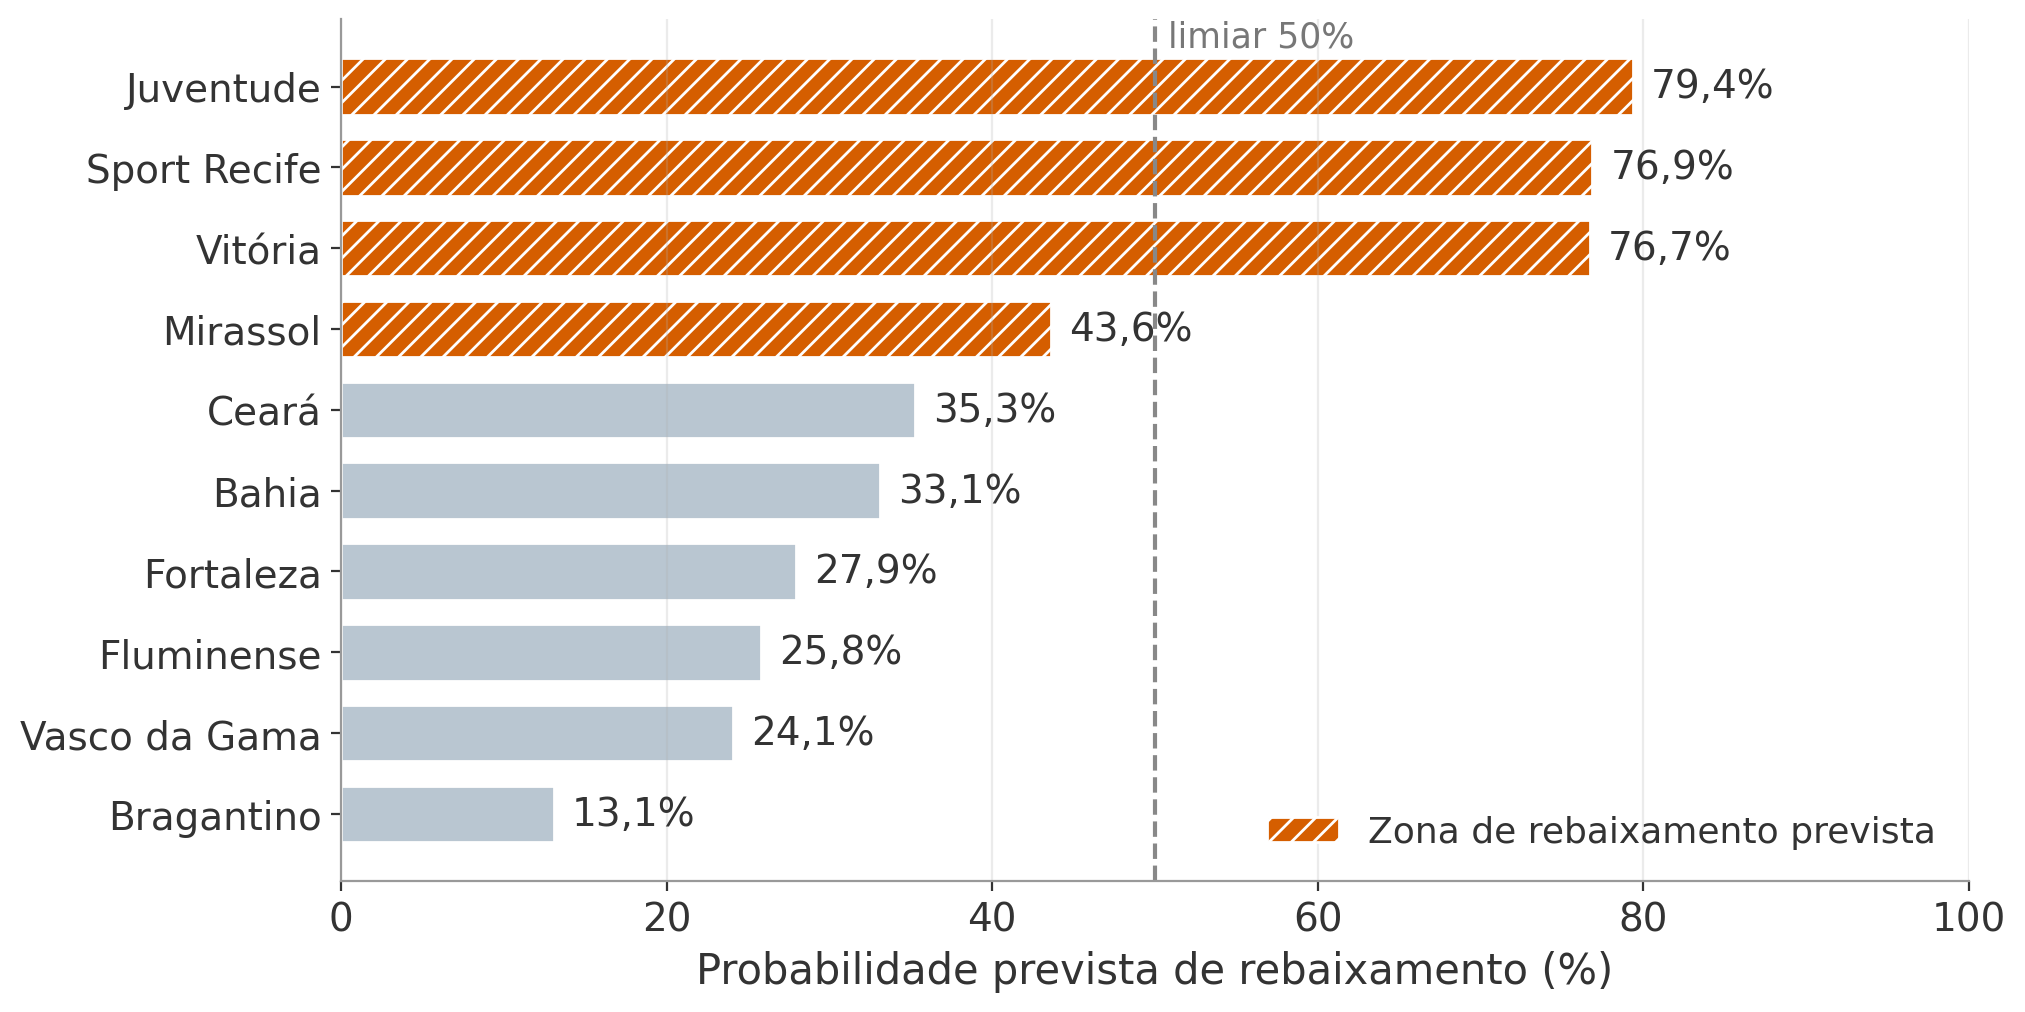
\includegraphics[height=0.62\textheight]{slide_previsao2025.png}
    \end{center}
    \begin{center}
        \small Juventude, Sport Recife, Vitória e Mirassol --- os quatro maiores riscos.
    \end{center}
\end{frame}

% ── 14. A prova real ───────────────────────────────────────────────────────
\begin{frame}{A prova real: o campeonato aconteceu}
    \framesubtitle{Validação retroativa contra o resultado oficial de 2025}
    \vspace{0.3cm}
    \begin{center}
        \tile{verm}{2 de 4}{rebaixamentos\par previstos no corte}\hfill
        \tile{azul}{0,922}{AUC-ROC realizado\par na temporada}\hfill
        \tile{azul}{4 de 4}{rebaixados entre os\par 7 maiores riscos}\hfill
        \tile{azul}{59/64}{pares ordenados\par corretamente}
    \end{center}

    \vspace{0.45cm}
    \begin{itemize}\itemsep0.25em
        \item Melhor AUC de todos os períodos avaliados --- acima do teste (0,828).
        \item O LightGBM, campeão no teste, caiu para \textbf{0,711}: a instabilidade
              vista no \emph{walk-forward} se confirmou.
        \item Supera as heurísticas ingênuas --- menor valor de elenco (0,906)
              e pior média de pontos (0,766).
    \end{itemize}
\end{frame}

% ── 15. Previsto x aconteceu ───────────────────────────────────────────────
\begin{frame}{Previsto \emph{versus} aconteceu}
    \vspace{0.1cm}
    \begin{center}
        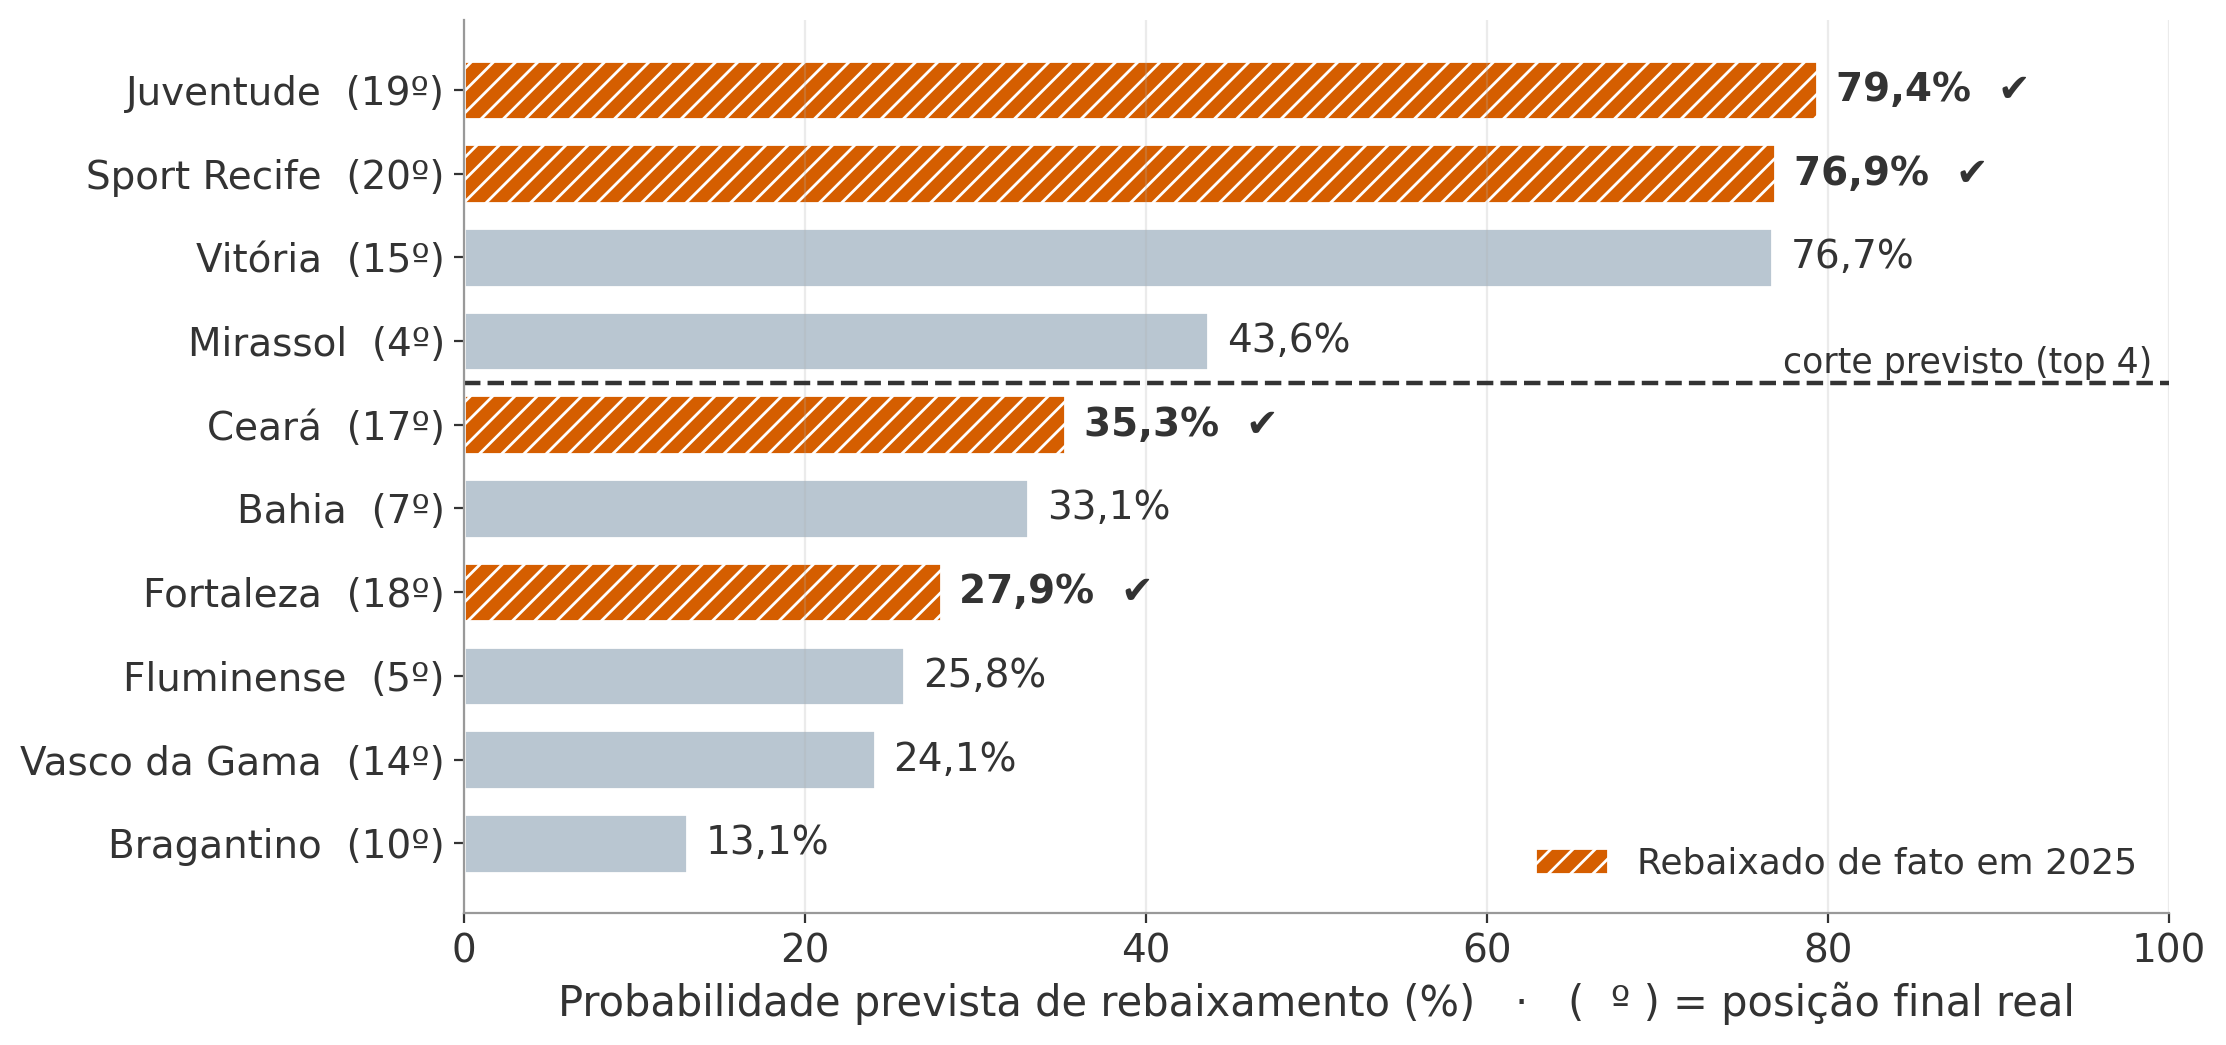
\includegraphics[height=0.64\textheight]{slide_validacao.png}
    \end{center}
    \begin{center}
        \small Os quatro rebaixados reais estão no \textbf{topo do ranking}.
    \end{center}
\end{frame}

% ── 16. O erro que ensina ──────────────────────────────────────────────────
\begin{frame}{O erro que mais ensina: Mirassol}
    \framesubtitle{Um caso atípico --- e o tempo tem dado razão ao modelo}
    \vspace{0.3cm}
    \begin{center}
        \tile{verm}{43,6\%}{risco previsto\par para 2025}\hspace{0.8cm}
        \tile{verde}{4.\textordmasculine{}}{posição final\par em 2025}\hspace{0.8cm}
        \tile{verm}{19.\textordmasculine{}}{em 2026, campeonato\par em curso}
    \end{center}

    \vspace{0.3cm}
    \begin{itemize}\small\itemsep0.25em
        \item Estreante sem histórico na Série A: as 12 \emph{features} de janela
              receberam a mediana do treino.
        \item Em 2026 o clube aparece na \textbf{zona de rebaixamento} --- a fragilidade
              apontada não desapareceu, apenas demorou uma temporada.
    \end{itemize}

    \vspace{0.35cm}
    \begin{center}
        \faixa{azul}{Mirassol é \emph{outlier}: sem a campanha atípica, teria caído.}
    \end{center}
\end{frame}

% ── 17. Visão longitudinal ─────────────────────────────────────────────────
\begin{frame}{Dez anos de risco em um quadro}
    \framesubtitle{Modelo retreinado só com o passado de cada temporada $\cdot$ recorte de 16 clubes}
    \vspace{0.1cm}
    \begin{center}
        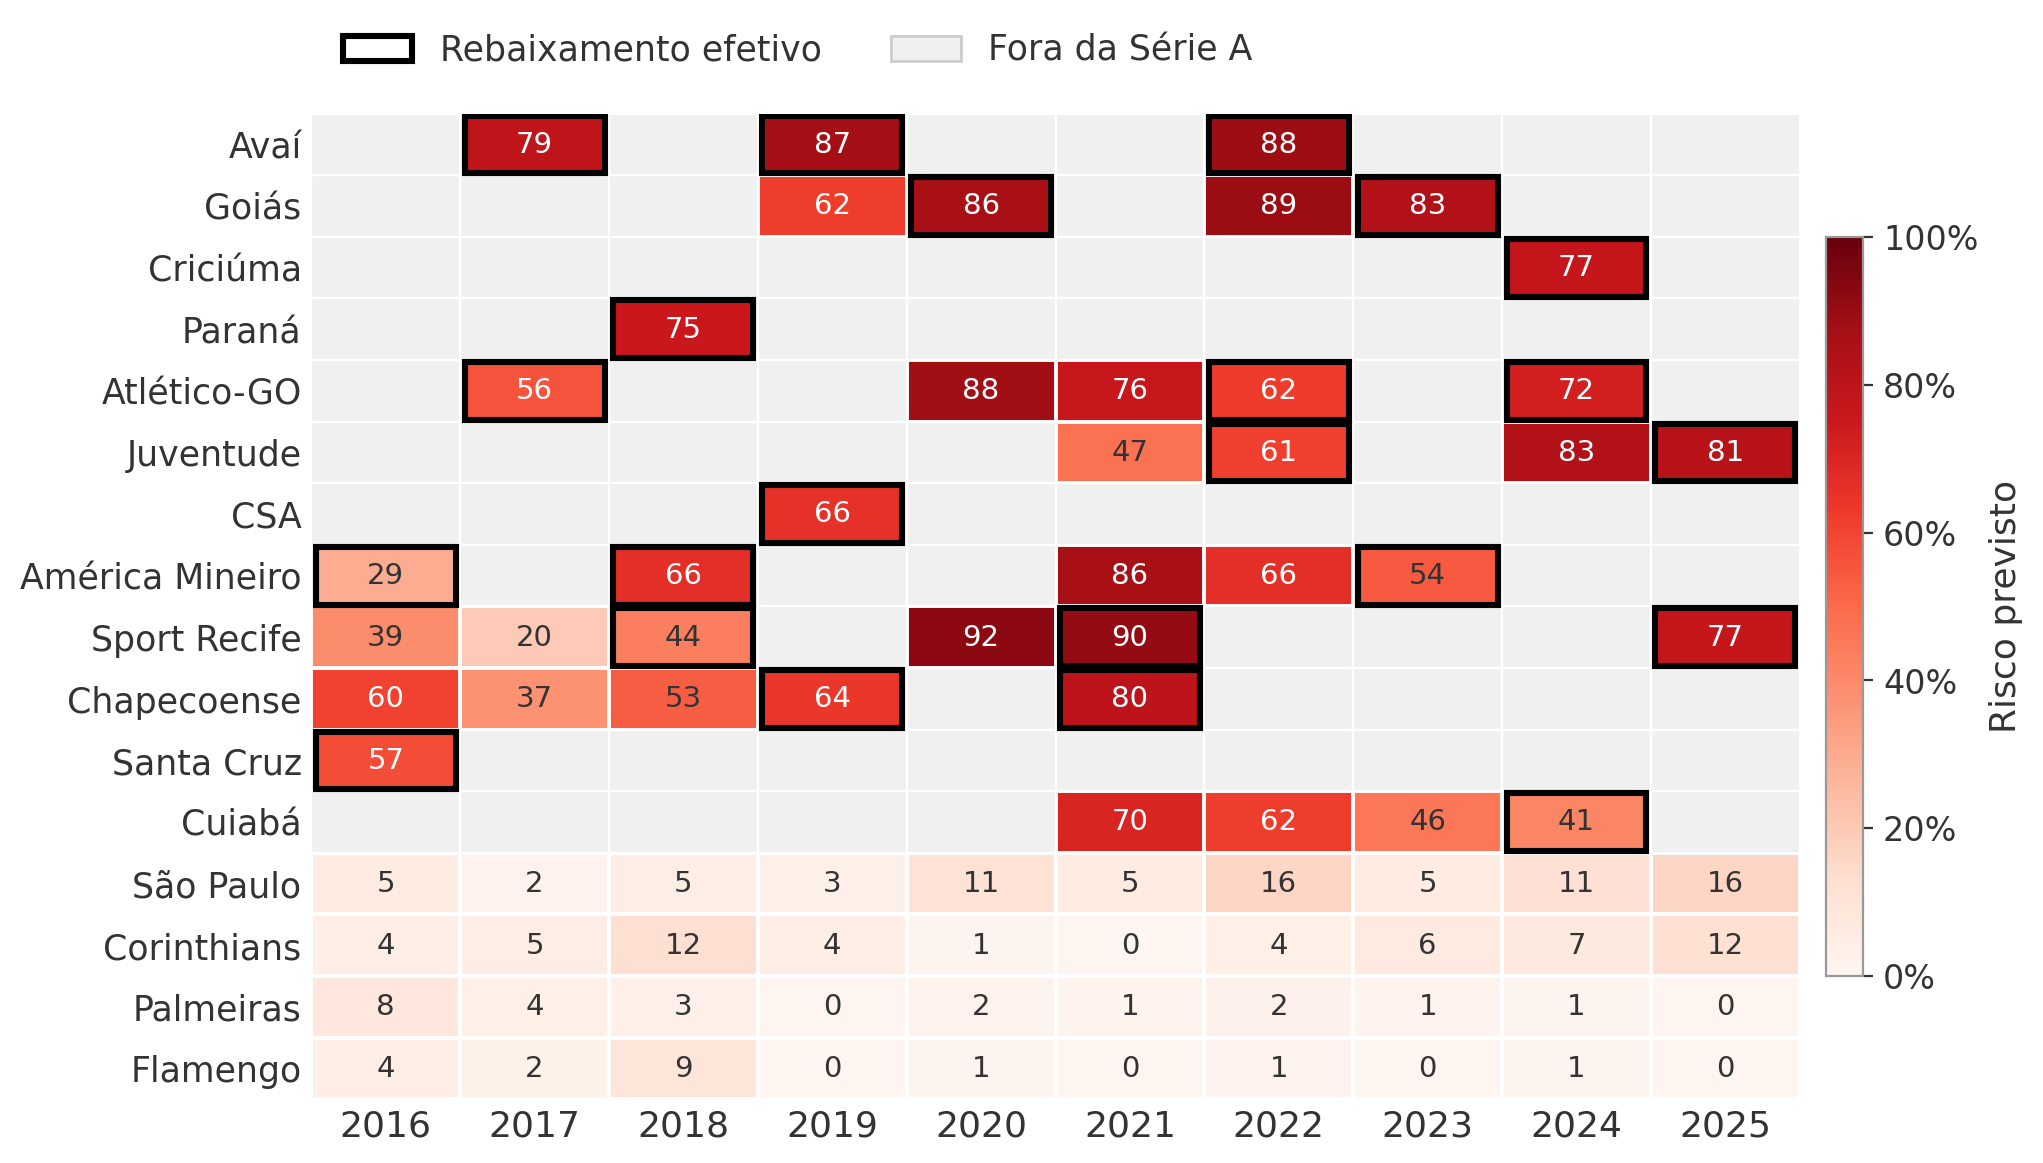
\includegraphics[height=0.63\textheight]{slide_heatmap.png}
    \end{center}
    \begin{center}
        \small O ``efeito elevador'' no topo; os grandes em risco baixo e estável embaixo.
    \end{center}
\end{frame}

% ── 18. Contribuições ──────────────────────────────────────────────────────
\begin{frame}{Contribuições}
    \vspace{0.6cm}
    \begin{enumerate}\itemsep0.7em
        \item[\textcolor{azul}{\textbf{1.}}] Um \emph{pipeline} \textbf{reprodutível} e sem
              vazamento temporal para previsão esportiva no contexto brasileiro.
        \item[\textcolor{azul}{\textbf{2.}}] A demonstração empírica da
              \textbf{armadilha da acurácia}: mesma acurácia, AUC de 0,652 contra 0,877.
        \item[\textcolor{azul}{\textbf{3.}}] Evidência de que o \textbf{histórico recente
              complementa} os indicadores financeiros de elenco.
        \item[\textcolor{verm}{\textbf{4.}}] Uma previsão \textbf{verificada contra a
              realidade} --- e não apenas prometida.
    \end{enumerate}
\end{frame}

% ── 19. Limites ────────────────────────────────────────────────────────────
\begin{frame}{Limites e próximos passos}
    \vspace{0.45cm}
    \begin{columns}[t]
        \begin{column}{0.47\textwidth}
            \textbf{\color{verm}Limitações}
            \begin{itemize}\small\itemsep0.2em
                \item só dados pré-temporada: não capta lesões, troca de técnico, calendário
                \item $\sim$220 observações --- amostra pequena
                \item recém-promovidos dependem da imputação
            \end{itemize}
        \end{column}
        \begin{column}{0.47\textwidth}
            \textbf{\color{azul}Trabalhos futuros}
            \begin{itemize}\small\itemsep0.2em
                \item retreino \textbf{durante} a temporada
                \item \emph{features} do mercado de transferências
                \item modelos sequenciais, com mais temporadas
                \item Série B e outras ligas
            \end{itemize}
        \end{column}
    \end{columns}

    \vspace{0.6cm}
    \begin{center}
        \fonte{Sensibilidade: imputação por média em vez de mediana $\to$ AUC 0,828 (igual); janelas de 2 e 4 temporadas $\to$ 0,836.}
    \end{center}
\end{frame}

% ── 20. Fecho ──────────────────────────────────────────────────────────────
\begin{frame}{}
    \vspace{1.1cm}
    \chave{O modelo previu antes.\\ O campeonato confirmou a ordenação.}

    \vspace{1.0cm}
    \begin{center}
        \faixa{verm}{Agora, a ferramenta em funcionamento: demonstração do aplicativo}
    \end{center}

    \vspace{0.9cm}
    \begin{center}
        \fonte{Código, dados e experimentos: \texttt{github.com/leonardofeitos4/previsao-tcc}}
    \end{center}
\end{frame}

% ── 21. Reserva ────────────────────────────────────────────────────────────
{
\setbeamertemplate{footline}{}
\begin{frame}[plain]
    \vspace{0.3cm}
    {\small\color{tinta2}\textbf{Reserva --- números de apoio}}

    \vspace{0.3cm}
    \scriptsize
    \begin{columns}[t]
        \begin{column}{0.47\textwidth}
            \textbf{\emph{Walk-forward} (médias)}\\
            Reg. Logística 0,794 $\pm$ 0,058\\
            Random Forest 0,762 $\pm$ 0,071\\
            LightGBM 0,700 $\pm$ 0,151\\
            XGBoost 0,659 $\pm$ 0,085

            \vspace{0.3cm}
            \textbf{\emph{Fold} 2020 (pandemia)}\\
            LightGBM 0,438 $\cdot$ XGBoost 0,531 $\cdot$ RL 0,703

            \vspace{0.3cm}
            \textbf{Teste 2023--2024 (XGB e LGBM idênticos)}\\
            3 acertos entre 8 rebaixados $\cdot$ 2 falsos positivos\\
            30 acertos de permanência

            \vspace{0.3cm}
            \textbf{Calibração (quartil de maior risco)}\\
            previsto 63,6\% $\cdot$ observado 50,0\%
        \end{column}
        \begin{column}{0.47\textwidth}
            \textbf{Base}\\
            220 obs. rotuladas $\cdot$ 20\% de prevalência\\
            15,5\% de ausentes nas janelas\\
            Elenco: média \euro55,3M $\cdot$ DP \euro38,5M $\cdot$ máx. \euro214,2M

            \vspace{0.3cm}
            \textbf{Desbalanceamento}\\
            \texttt{class\_weight='balanced'} (RL, RF, LGBM)\\
            \texttt{scale\_pos\_weight=4} (XGBoost)

            \vspace{0.3cm}
            \textbf{Otimização}\\
            RandomizedSearchCV, 30 candidatos,\\
            TimeSeriesSplit de 5 \emph{folds}, critério AUC

            \vspace{0.3cm}
            \textbf{Rebaixados de 2025}\\
            Sport (20.\textordmasculine{}) $\cdot$ Juventude (19.\textordmasculine{})\\
            Fortaleza (18.\textordmasculine{}) $\cdot$ Ceará (17.\textordmasculine{})
        \end{column}
    \end{columns}
\end{frame}
}

\end{document}
